\documentclass[../full_thesis/full_thesis.tex]{subfiles}

% Default image directory
\newcommand{\thisdir}{../analytic_timing_noise_cgw}
\graphicspath{{\thisdir/img/}}

\begin{document}

It's unclear at this time what causes timing noise, but from Chapter.~\ref{sec:
timing noise in cgw} we know that it may pose a problem for continuous GW
searches if the phase evolution is effected by timing noise and that is not
included in the search templates. In addition to searches for isolated neutron
stars, searches for GWs from low-mass X-ray binary systems (LMXBs) may
experience similar difficulties due to stronger form of timing noise known as
`spin-wandering', which constrains the maximal coherence time to the order of a
few days before it would lead to a complete loss of SNR, thereby limiting the
best achievable sensitivity \citep[see][for
details]{ligo2015scox1,leaci2015,ScoX1:MDC1}.

Ideally, we would like to be able to predict when searches are at risk to
timing noise.  We have already done this in Chapter.~\ref{sec: timing noise in
cgw} by using an empirical description of timing noise from the Crab pulsar.
However, this is limiting as the way timing noise manifests varies between
sources. An alternative method is to model timing noise, predict the form of
the continuous GW signal and then calculate the mismatch. In this chapter, we
will do this for the random walk model of timing noise as described in
Section~\ref{sec: TN interpretations random walk models}.  Recent observations
\citep{Hobbs2010} suggest that such a description does not capture the physics
of timing noise in isolated radio pulsars and hence is not a useful way to
infer neutron star physics. Nevertheless, empirically the timing residuals of
many pulsars are indistinct from a random walk, so while it cannot help with
inference, it is a useful description if we only need to know what timing noise
`looks like'. Moreover, the random walk model can also be applied to LMXBs
where the amount of spin-wandering could be inferred from fluctuations in the
luminosity. We will not apply the model to make such predictions in this
chapter, but we will calculate the mismatch given the random walk model.


\section{Defining a random walk}
\label{sec: Defining a random walk}
To calculate the fully-coherent mismatch, we will model the random walk as a
zero-mean gaussian walk in the phase, frequency, and spin-down which occurs at
$\Nsd$ fixed time intervals, $\Delta T$ such that the total observation time is
$\Tobs = \Nsd \Delta T$.
This allows us to write the signal as 
a peicewise Taylor expansion with $N$ subdomans. Choosing fixed time intervals appears to
introduce an additional timescale not usually present in random walk models.
However, as discussed in Appendix~\ref{sec: physical interpretation of the monthly
ephemeris} this is consistent with a large number of unresolved events which
are measured over a fixed timescale.

In this model, the spin-down rate will be the highest order term
which undergoes a random walk. Therefore, between the $i$ and $i-1$ subdomains
we may write the difference between the signal and template (defined in
Eqn.~\eqref{eqn: Delta Phi}) as
\begin{equation}
\Delta \fdot_{i} - \Delta\fdot_{i-1} = \tn \fdot_{i} \sim \mathcal{N}(0, \sigS),
\end{equation}
where $\mathcal{N}$ denotes the normal distribution and we have defined $\sigS$
as the standard-deviation of the step sizes in the spin-down rate. The residual
between parameter space offsets is denoted by $\tn$ which is normally
distributed. Rearranging this gives an expression for the offset in the
$i^{th}$ subdomain, by induction we can also write down the $i-1$ term
\begin{align}
\Delta\fdot_{i} &  = \tn\fdot_{i} + \Delta\fdot_{i-1}  \\
\Delta\fdot_{i-1} &  = \tn\fdot_{i-1} + \Delta\fdot_{i-2}  .
\end{align}
Let us start each random walk from the origin (we will return to this point in 
Sec.~\ref{sec: Random walk models part II}), then
as each step proceeds from the previous step, we have that
\begin{equation} 
\Delta\fdot_{i} = \s{j=1}{i}\tn\fdot_{j}.
\label{eqn: delta fdot n} 
\end{equation}

To illustrate this, in Fig.~\ref{fig: Illustration fdot int} we plot an example
of a random walk in spin-down as given by Eqn.~\eqref{eqn: delta fdot n}.
\begin{figure}[ht]
\centering
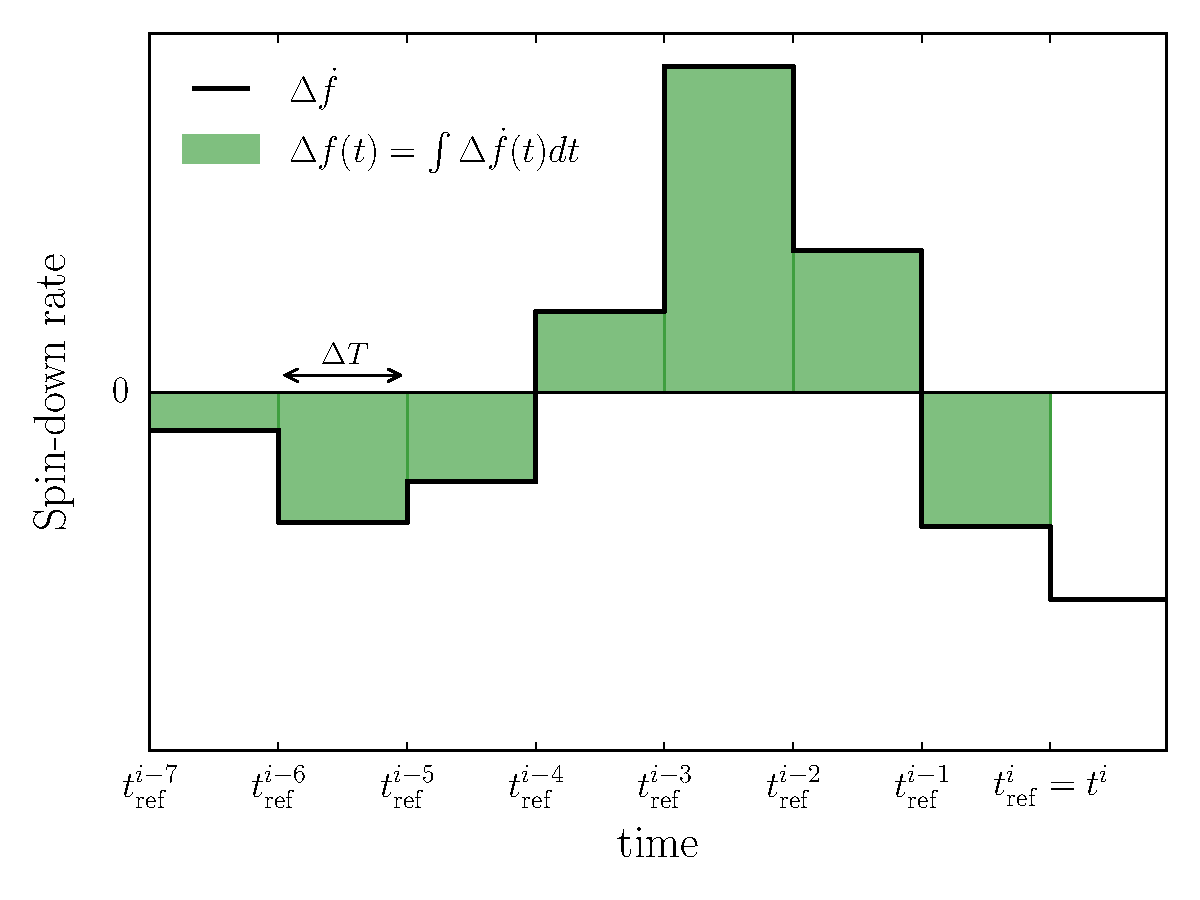
\includegraphics[width=0.7\textwidth]{Illustration_F1_int}
\caption{An example of a random walk in the spin-down rate, 
Eqn.~\eqref{eqn: delta fdot n}. The filled green blocks indicate the
summation defined in Eqn.~\eqref{eqn: f offset induced} required to
calculate the induced change in frequency at $t^{i}$ due to the random walk in
spin-down rate.}
\label{fig: Illustration fdot int}
\end{figure}

If we want to model a random walk in the phase, frequency, and spin-down rate
concurrently, then we must consider the effect that a
random walk in spin-down will have on the frequency and phase. For example, if we
increase the spin-down rate for a period of time, then we would expect the frequency
to decrease at a greater rate during this period. In our discreet model, it is
not possible to dynamically change the frequency during a single subdomain.
However, we can approximate this by updating the frequency in the next
subdomain with the induced frequency offset due to the spin-down in previous
subdomains. This must be done for the induced effect from the random walk in spin-down rate on
the phase and frequency, and for the induced effect from the random walk in frequency
on the phase. There is induced effect for the spin-down rate: the effect only
propagates to lower order terms.

Because the random walk is discreet and constant in any given subdomain, we can
calculate the offset in the lower order terms from a Taylor expansion. The
total offset at the  $i^{th}$ reference time is then given by the summation of
the offset caused by all higher order terms up to that reference time. The
reference times can be arbitrarily chosen, but setting each to start at the
beginning of the subdomain simplifies the calculation. 
The frequency offset induced by the spin-down can be
calculated using a Taylor expansion
\begin{equation}
\Delta \f_{i} = \s{j=1}{i-1}\Delta\fdot_{j} \dT .
\label{eqn: f offset induced} 
\end{equation}
This can be though of as the integration of the spin-down up to the $i^{th}$
reference time and is illustrated by the green blocks in Fig.~\ref{fig:
Illustration fdot int}. 

Since we want to consider random walks in all three parameters we now add in a
random walk in frequency. Each step is independent of the induced effect from
the spin-down and is given by \mbox{$\tn \f_{i} \sim \mathcal{N}(0, \sigF)$}. The two
effects will sum linearly such that the frequency offset is
\begin{equation}
\Delta \f_{i} = \s{j=1}{i}\tn \f_{j} + \s{j=1}{i-1}\Delta\fdot_{j} \dT.
\label{eqn: f offset} 
\end{equation}

By a similar process we can calculate the induced effect of the frequency and
spin-down on the phase. Including the random walk in the phase
for which $\delta \phi_i \sim \mathcal{N}(0, \sigP)$, the phase offset is given by
\begin{equation}
\Delta\phi_{i}  =  \s{j=1}{i}\tn \phi_{j} 
+ 2\pi\left(\s{j=1}{i-1}\Delta \f_{j}\dT 
+ \frac{1}{2}\s{j=1}{i-1}\Delta \fdot_{j}\dT^{2}\right).
\label{eqn: phi offset}
\end{equation}

%Equations \eqref{eqn: f offset} and \eqref{eqn: phi offset} will allows us to
%construct the parameter space offsets in all three terms from the distibutions
%$\tn \phi_i$, $\tn \phi_i$, and $\tn \phi_i$.




\section{Random walk models part I}
\label{sec: Random walk models part I}
We will now calculate the mismatch for a fully-coherent search given the
random walk in phase, frequency, and spin-down rate defined in the previous
section.

Let us begin by expanding the metric-mismatch summation from Eqn.~\eqref{eqn:
mismatch}.  Writing the summations explicitly, we have
\begin{align}
\mutilde & = g_{\alpha\beta i j}\dl^{\alpha i}\dl^{\beta j}  \\
&=\s{i=1}{\Nsd}\s{j=1}{\Nsd}g_{\alpha\beta i j}\dl^{\alpha i}\dl^{\beta j}  \\
&= \s{i=1}{\Nsd}g_{\alpha\beta i i}\dl^{\alpha i}\dl^{\beta i}
+ \s{i=1}{\Nsd} \s{\substack{j=1\\ j \ne i}}{\Nsd} g_{\alpha \beta ij}\dl^{\alpha i}\dl^{\beta j}.
\end{align}
The summation has been intentionally split into terms for which the two
subdomains are the same and those for which they are different. The metric when
the reference time is at the beginning of each subdomain is given by
Eqn.~\eqref{eqn: metric equal subdomains tref 0}. By considering the metric for
the two cases, we can write the two distinct components as
\begin{equation}
g_{\alpha\beta ij} = \left\{
\begin{array}{cc}
g_{\alpha\beta}^{\mathrm{E}} & \textrm{ if } i =j \\
g_{\alpha\beta}^{\mathrm{NE}} & \textrm{ if } i  \ne j
\end{array}\right.  .
\end{equation}
Then the fully-coherent metric-mismatch can be calculated from
\begin{align}
\mutilde &= \s{i=1}{\Nsd}g_{\alpha\beta}^{\mathrm{E}}\dl^{\alpha i}\dl^{\beta i}
+ 2\s{i=1}{\Nsd} \s{j=1}{i-1} g_{\alpha \beta}^{\mathrm{NE}}\dl^{\alpha i}\dl^{\beta j} .
\label{eqn: mismatch sep}
\end{align}

\subsection{Writing the parameter offsets in terms of normal distributions}
Equations~\eqref{eqn: f offset} and \eqref{eqn: phi
offset} give the offsets as functions of the offsets in higher order
parameters. In order to calculate statistical values, we now write these in terms of
the normal distributions from which the random walks are constructed.
Substituting Eqn.~\eqref{eqn: delta fdot n} into Eqn.~\eqref{eqn: f offset} and using the summation properties defined
in Appendix~\ref{sec: summation identities}, we have
\begin{align}
\Delta \f_{i}  & = \s{j=1}{i}\tn \f_{j}
+ \s{j=1}{i-1}\s{k=1}{j}\tn \fdot_{k} \dT ,  \\
& = \s{j=1}{i}\tn \f_{j}
+ \s{j=1}{i-1}(i-j)\tn \fdot_{j} \dT .
\label{eqn: delta f n}
\end{align}
Similarly, substituting this equation into Eqn.~\eqref{eqn: phi offset} we
have
\begin{align}
\begin{split}
\Delta\phi_{i} & = \s{j=1}{i}\tn \phi_{j}
+ 2\pi \left(\s{j=1}{i-1}\Delta\f_{j}\dT
+ \frac{1}{2}\s{j=1}{i-1}\Delta\fdot_{j}\dT^{2}\right) \\
& = \s{j=1}{i}\tn \phi_{j} + 2\pi\left(\s{j=1}{i-1}\left(\s{k=1}{j}\tn\f_{k}
+ \s{k=1}{j-1}(j-k)\tn\fdot_{k}\dT\right)\dT
 + \frac{1}{2}\s{j=1}{i-1}\s{k=1}{j}\Delta\fdot_{k}\dT^{2} \right)  \\
& = \s{j=1}{i}\tn \phi_{j} + 2\pi\left(\s{j=1}{i-1}(i-j)\tn\f_{j}\dT
 + \s{j=1}{i-1}\s{k=1}{j-1}(j-k)\tn\fdot_{k}\dT^{2}
 + \frac{1}{2}\s{j=1}{i-1}(i-j)\Delta\fdot_{j}\dT^{2} \right)  \\
& = \s{j=1}{i}\tn \phi_{j} + 2\pi\left(\s{j=1}{i-1}(i-j)\tn\f_{j}\dT
 + \frac{1}{2}\s{j=1}{i-1}\left(\left(i-j\right)\left(i-j-1)\right)
 + (i-j)\right)\tn\fdot_{j}\dT^{2}\right)  \\
& = \s{j=1}{i}\tn \phi_{j} + 2\pi\left(\s{j=1}{i-1}(i-j)\tn\f_{j}\dT
 + \frac{1}{2}\s{j=1}{i-1}(i-j)^{2}\tn\fdot_{j}\dT^{2}\right)
\end{split}
\label{eqn: delta phi n}
\end{align}

\subsection{Taking the expectation}

In Eqn.~\eqref{eqn: delta fdot n}, Eqn.~\eqref{eqn: delta f n},
Eqn.~\eqref{eqn: delta phi n} we have written the parameter space offsets
(which are to be used in calculating the mismatch) purely in terms of the
random walk distributions $\tn \phi_i$, $\tn \f_i$, and $\tn \fdot_i$. We can
calculate the mismatch exactly given a set of random walk jumps by inserting
these into Eqn.~\eqref{eqn: mismatch sep}. However, since we are dealing with
statistical quantities, we can instead infer the behaviour of the mismatch
under the random walk by taking an expectation.

Inserting Eqn.~\eqref{eqn: delta fdot n}, Eqn.~\eqref{eqn: delta f n},
Eqn.~\eqref{eqn: delta phi n}  in Eqn.~\eqref{eqn: mismatch sep} yields a
number of terms with all the permutations of two terms from $[\tn \phi, \tn \f,
\tn \fdot]$. Taking the expectation, all the cross-correlated terms, such as
$\tn\phi_{i}\tn \fdot$, will have an expectation of zero since the steps of the
random walk are independent. The only non-vanishing terms are given by
\begin{align}
E[\tn\phi_{i}\tn\phi_{j}] &= \delta_{ij}\sigP, &
E[\tn\f_{i}\tn\f_{j}] &= \delta_{ij}\sigF,&
E[\tn\fdot_{i}\tn\fdot_{j}] &= \delta_{ij}\sigS,
\end{align}
After some simplification we find that the mismatch is given by
\begin{align}
\begin{split}
E[\mutilde]   = &  \frac{A_{\phi}}{6} \left(\Nsd - \frac{1}{\Nsd}\right)
+ \frac{\pi^{2} A_{{f}}}{30}\left(4 \Nsd^{3} + 5 \Nsd^{2} + \frac{1}{\Nsd}\right)\\
 & +  \frac{\pi^{2} A_{{\dot{f}}}}{3780} \left(66 \Nsd^{5} - 21 \Nsd^{3} + 105 \Nsd^{2}
 + 217 \Nsd + 63 - \frac{94}{\Nsd}\right),
\end{split}
\label{eqn: expectation}
\end{align}
where
\begin{equation}
	A_{\phi} = \sigP \;\;\;\;\;
    A_{\f} = \sigF\Delta T^{2} \;\;\;\;\;
    A_{\fdot} = \sigS\Delta T^{4},
\end{equation}
define three `activity parameters'.

Recalling that $\Nsd=\Tobs/\Delta T$, Eqn.~\eqref{eqn: expectation} makes
predictions for the leading order
scaling of the three random walks with the observation period
\begin{equation}
E[\mutilde]_{\mathrm{PN}} \sim \sigP \frac{\Tobs}{\Delta T}, \hspace{10mm}
E[\mutilde]_{\mathrm{FN}} \sim \sigF \frac{\Tobs^{3}}{\Delta T}, \hspace{10mm}
E[\mutilde]_{\mathrm{SN}} \sim \sigS \frac{\Tobs^{5}}{\Delta T}.
\label{eqn: scalings}
\end{equation}

These results are a function both of the observation span $\Tobs$ and the
random walk model parameters $\sigP, \sigF, \sigS$ and $\Delta T$. In
Appendix~\ref{sec: physical interpretation of the monthly ephemeris}, we showed
that for a compound Poisson process random walk, the variance after a duration
$\Delta T$ scaled as $\sigma^{2} \propto \Delta T$. This means that the leading
order scalings in Eqn.~\eqref{eqn: scalings} are insensitive to how the random
walk is parameterised: changing $\Delta T$ produces a corresponding change in
$\sigma^{2}$ such that the leading order mismatch remains the same for a fixed
observation time.

\subsection{Verifying the results}

We can observe the leading order scaling of Eqn.~\eqref{eqn: scalings}
directly and verify the predictions made by Eqn.~\eqref{eqn: expectation} by
comparing with exact numerical results. That is, using the signal injection and
recovery tools developed in Section~\ref{sec: narrow-band method} of
Chapter.~\ref{sec: timing noise in cgw} we simulate signals undergoing a random
walk and calculate the corresponding mismatch (no minimisation step is done
here, this is discussed in the next section). In particular, we perform three
Monte Carlo studies for a random walk in the phase, frequency, and spin-down
rate and in each case compare the simulated results with the analytic
prediction. The results are shown in Figure~\ref{fig: rw I} and demonstrate good
agreement between the simulation means and the prediction of Eqn.~\eqref{eqn:
expectation}.

\begin{figure}[ht]
\centering
\subfloat[Random walk in phase]{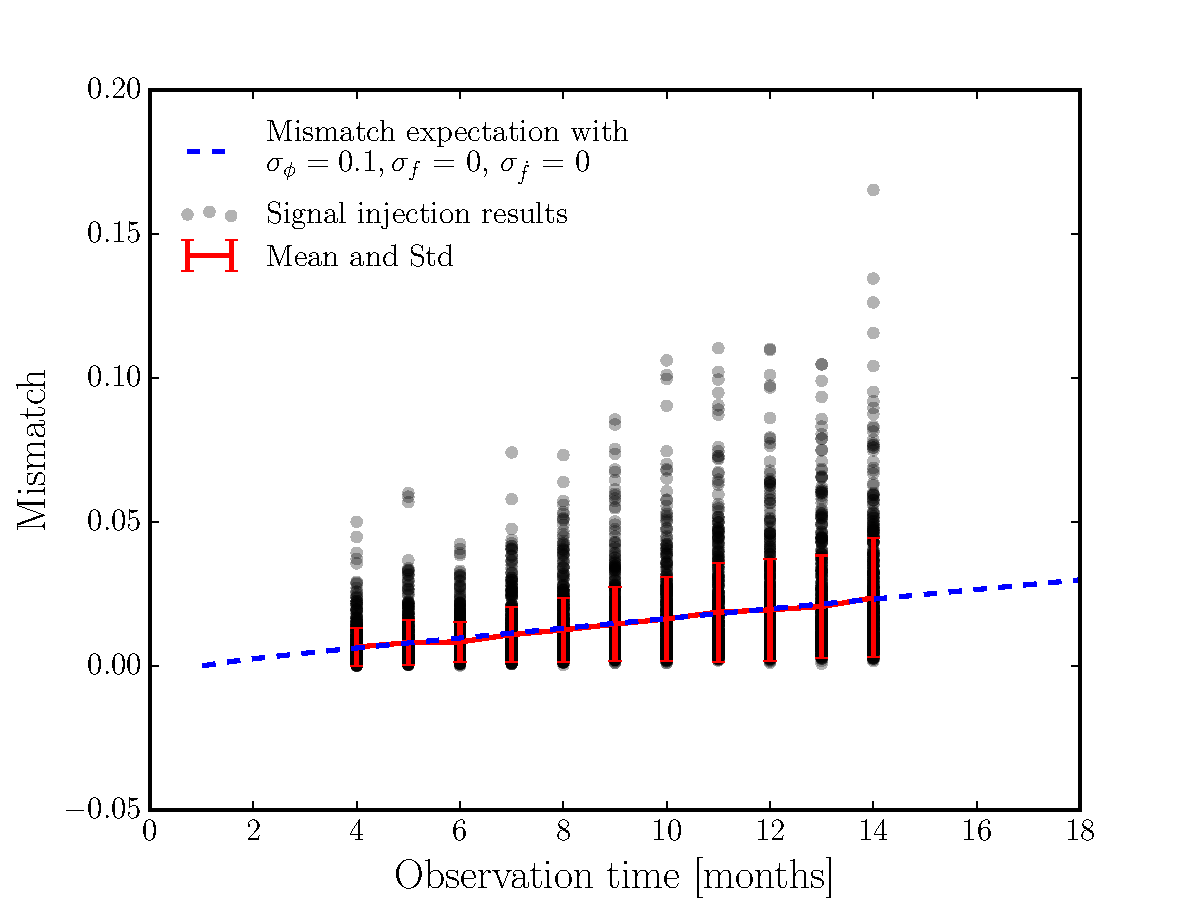
\includegraphics[width=0.5\textwidth]{ExpectationPhase}}
\subfloat[Random walk in frequency]{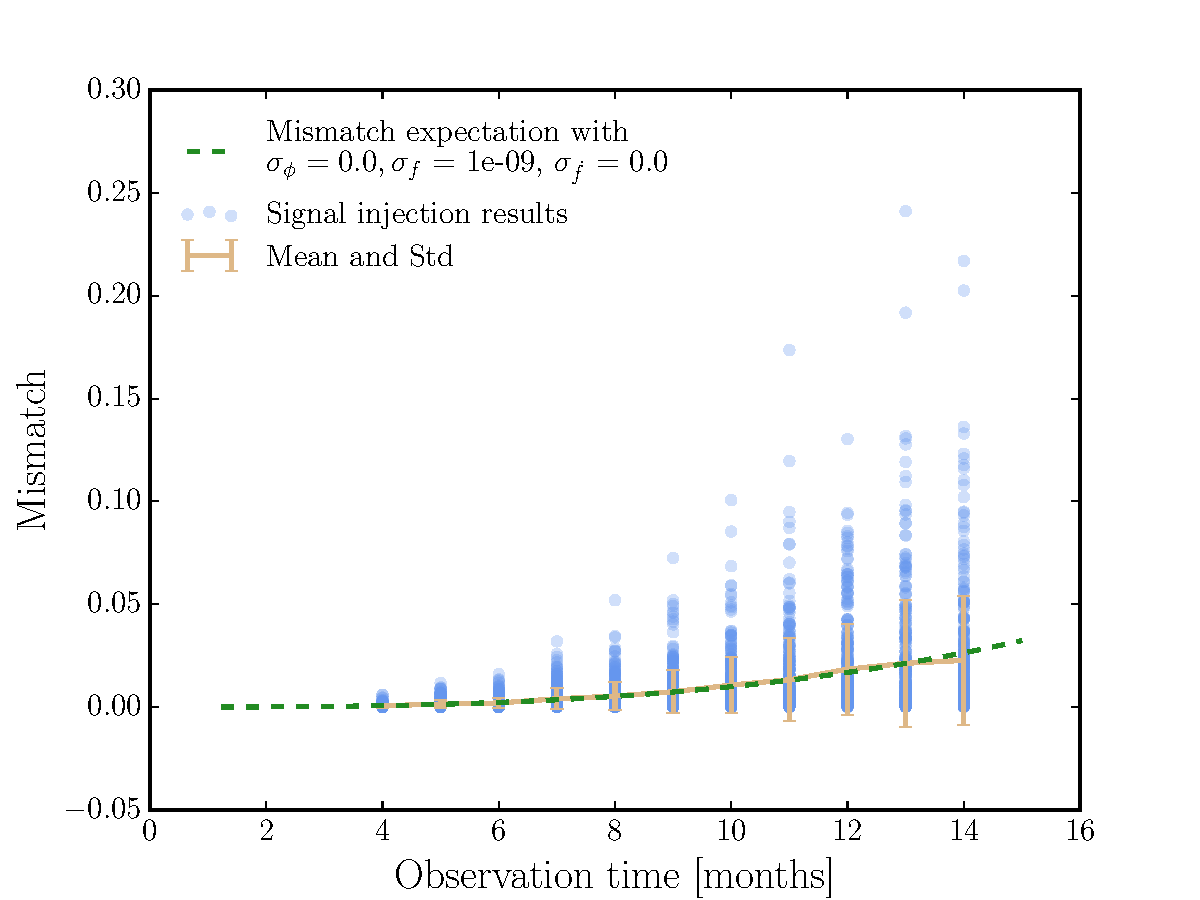
\includegraphics[width=0.5\textwidth]{ExpectationFrequency}}\\ \subfloat[Random walk in spin-down]{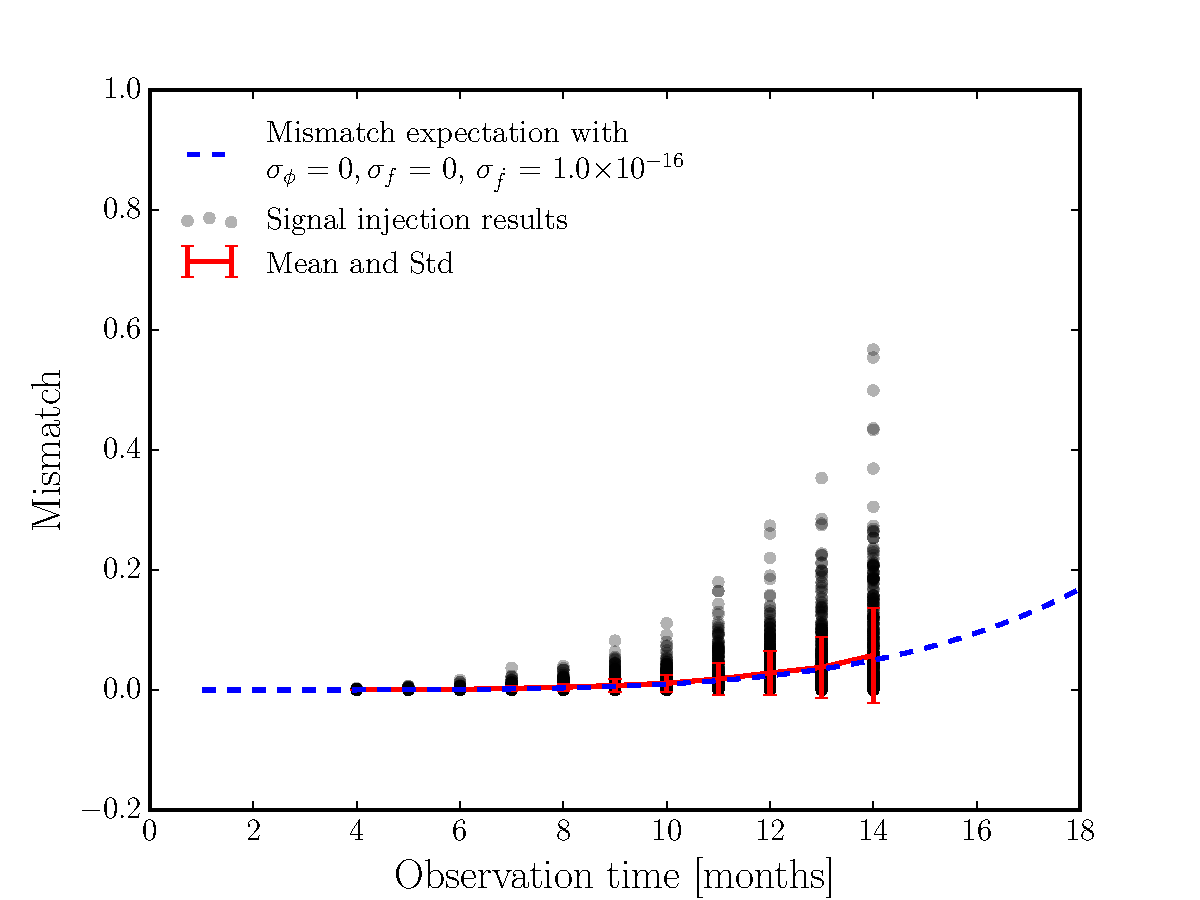
\includegraphics[width=0.5\textwidth]{ExpectationSpindown}}
\caption{A comparison of Monte Carlo numerical simulated mismatch with the prediction
of Eqn.~\eqref{eqn: expectation} for a random walk in the phase, frequency,
and spin-down rate.}
\label{fig: rw I}
\end{figure}

\subsection{Implied scalings}



\section{Random walk models part II} 
\label{sec: Random walk models part II}
In Section~\ref{sec: Defining a random walk} we have defined a random walk
model for which we subsequently calculated the fully-coherent mismatch in
Section~\ref{sec: Random walk models part I}. However, this is a special case
in which the random walk for each parameter offset (the difference between the
signal and the template) begins at the origin and then grows with time. It is
the signal which undergoes a random walk, so in this case we have set the
template to exactly match the signal and $t=0$. However, one could imagine choosing
the template in a different way which would reduce the overall mismatch; as such
Eqn.~\eqref{eqn: expectation} may overestimate the mismatch. The proper thing to
do is to minimise the mismatch with respect to the
template parameters~$\lt^{\alpha}$ which are implicitly in the calculation of
Section~\ref{sec: random walk models part I} through
\begin{align}
\Delta \lambda^{\alpha i} = \ls^{\alpha i} - \lt^{\alpha i},
\end{align}
as first defined in Section~\ref{sec: generalising the metric mismatch}.

Ideally, we would like to repeat the calculation leading to Eqn.~\eqref{eqn:
expectation} minimising the mismatch with respect to the template parameters.
However, this calculation has not yet been peformed so a practical alternative
method which we will use here is to begin with the random walk starting at the
origin, as defined in Section~\ref{sec: Defining a random walk}, and then fit and
remove a polynomial of degree $k$. This leaves us with a residual random walk for
which we then compute the mismatch. We will then verify that this captures the
essential features of minimising the mismatch by comparing with numerical
simulations in which the exact mismatch is minimised numerically.

In Appendix~\ref{sec: least squares minimisation of a random walk}, we
introduce the basic tools of least squares fitting and removing a polynomial of
degree $k$ to a generic random walk. In the following sections, we will
calculate the minimised mismatch for random walks in the phase or frequency; we
have not yet calculated the corresponding result for mixtures or random walks
in the spin-down rate. We have a choice in the degree of polynomial to fit and
remove. Since most searches minimise the mismatch with respect to the template
frequency $f_\textrm{t}$ and spin-down rate $\dot{f}_{\textrm{t}}$, this is
equivalent to fitting and removing a $k=2$ polynomial to the phase residual.

\subsection{Random walk in the phase}
\label{sec: minimised rw in phase}
We begin with the simplest case of a random walk in phase, for which we have
\begin{equation}
\Delta\phi_{i} = \s{j=1}{i}\mathcal{N}(0, \sigP).
\end{equation}
Then, as shown in Eqn.~\eqref{eqn: E yiyi} of Appendix~\ref{sec: least squares
minimisation of a random walk}, we have that
\begin{equation}
E[\Delta\phi_{i} \Delta\phi_{j}] = \sigP \min(i, j).
\end{equation}

Then, we define the residual difference between the signal and template
after fitting and removing a $2^{nd}$ order polynomial, $\hat{y}_i^{(2)}$, as
\begin{align}
\Delta^{(2)}\phi_i = \Delta\phi_i - \hat{y}_i^{(2)}.
\label{eqn: D2phi}
\end{align}
Note that the superscript `(2)' indicates the degree of polynomial and by
$\Delta^{(2)}\phi_i$ we mean the residual difference between the signal and
template after fitting and removing the polynomial.

We set the difference between the signal and template in all other parameters
to zero such that the mismatch for a random walk in the residual phase is
therefore
\begin{align}
\mutilde & = g_{0 0 i j} \Delta^{(2)}\phi^{i}\Delta^{(2)}\phi^{j} \\
& = \s{i=1}{\Nsd}g_{00}^{E} \Delta^{(2)}\phi_{i}\Delta^{(2)}\phi_{i}
+ 2 \s{i=1}{\Nsd}\s{j=1}{i-1}g_{00}^{NE}\Delta^{(2)}\phi_{i}\Delta^{(2)}\phi_{j}.
\label{eqn: 4202540871}
\end{align}
To calculate the expectation of the mismatch, we need to evaluate the
expectation of
\begin{align}
\Delta^{(2)}\phi_{i}\Delta^{(2)}\phi_{i} = & \left(\Delta\phi_{i}
- \s{k=1}{\Nsd}\CT_{ik}\Delta\phi_{k}\right)
 \left(\Delta\phi_{j} - \s{l=1}{\Nsd}\CT_{jl}\Delta\phi_{l}\right) \\
= & \Delta\phi_{i}\Delta\phi_{j} -
\left(\s{k=1}{\Nsd}\CT_{ik} \Delta\phi_{j}\Delta\phi_{k}
+ \s{l=1}{\Nsd}\CT_{jl}\Delta\phi_{i}\Delta\phi_{l}\right) \nonumber \\
& +
\s{k=1}{\Nsd}\s{l=1}{\Nsd}\CT_{ik}\CT_{jl} \Delta\phi_{k}\Delta\phi_{l},
\end{align}
where $\CT_{ij}$ is defined in Eqn.~\ref{eqn: C_2} and Eqn.~\ref{eqn:  MCC_2}
of Appendix~\ref{sec: least squares minimisation of a random walk} and we have
replaced $\Delta x$ with the time $\dT$. Then taking the expectation
\begin{align}
\E{\Delta^{(2)}\phi_{i}\Delta^{(2)}\phi_{i}} & =
%E\left[\Delta\phi_{i}\Delta\phi_{j}\right] -
%\left(\s{k=1}{\Nsd}E[\Delta\phi_{j}\Delta\phi_{k}]
%+ \s{l=1}{\Nsd}E[\Delta\phi_{i}\Delta\phi_{l}]\right) +
%\s{k=1}{\Nsd}\s{l=1}{\Nsd}E[\Delta\phi_{k}\Delta\phi_{l}]\\
%& = 
\sigma^{2}_{\phi} \left(\min(i, j) - \left(\s{k=1}{\Nsd}\CT_{ik} \min(j, k)
+ \s{l=1}{\Nsd}\CT_{jl}\min(i, l) \right)\right. \notag \\
& \hspace{13mm} \left. + \s{k=1}{\Nsd}\s{l=1}{\Nsd}\CT_{ik}\CT_{jl}\min(k, l)\right).
\label{eqn: expected mismatch dP0idP0j_k2}
\end{align}
Using symbolic mathematics packages we
calculate an analytic expression which is a function of $\dT, i, j$ and $\Nsd$.
Inserting this into Eqn.~\eqref{eqn: 4202540871} and simplifying we find that
\begin{align}
E[\mutilde]  & = \s{i=1}{\Nsd}g_{00}^{E} E\left[\Delta^{(2)}\phi_{i}\Delta^{(2)}\phi_{i}\right]
+ 2 \s{i=1}{\Nsd}\s{j=1}{i-1}g_{00}^{NE}E\left[\Delta^{(2)}\phi_{i}\Delta^{(2)}\phi_{j}\right]  \\
& = \frac{1}{70}\sigP\left(3N - \frac{27}{\Nsd}\right).
\label{eqn: Expected mismatch RW in phase k2}
\end{align}
This expression can be compared to Eqn.~\eqref{eqn: expectation} ignoring the
effect of the random walk in spin-down rate. Notably, we retain the same
leading order scaling of $\Nsd$, but the overall coefficient is decreased.
Rearranging the expression in the bracket demonstrates the mismatch is negative
or zero for $1 \ge \Nsd \ge 3$: this is a reflection of the minimum number of
points needed in order to perform the quadratic fit. This is shown later in
Sec.~\ref{sec: appendix conclusions} for the simpler case of fitting and
removing a polynomial from a generic random walk.

\subsection{Random walk in the frequency}

For a random walk in the frequency we have an added complexity caused by the
effect the frequency offsets induces in the phase. For the frequency offset we
have
\begin{align}
\Delta f_{i} &= \s{j=1}{i}\mathcal{N}(0, \sigF).
\end{align}
Recalling that we set the reference time at the beginning of each subdomain,
then as in Section~\ref{sec: Defining a random walk}, the induced phase offset is
\begin{align}
\Delta\phi_{i} &=2\pi \s{j=1}{i-1}\Delta f_{j}\dT \\
 & = 2\pi\dT \s{j=1}{i-1}\s{k=1}{j}\mathcal{N}(0, \sigF) \\
& = 2\pi\dT \s{j=1}{i}(i-j)\mathcal{N}(0, \sigF).
\label{eqn: P2F}
\end{align}
Note that we do not include a random walk in the phase here.

Then we calculate the expected values of combinations of the parameter space
offsets
\begin{align}
E[\Delta\f_{i}\Delta\f_{j}] & = \sigF \min(i, j), \label{eqn: E1} \\
E[\Delta\phi_{i}\Delta\f_{j}] & = 2 \pi \dT \sigF \s{k=1}{\min(i, j)}(i-k), \label{eqn: E2}\\
E[\Delta\phi_{i}\Delta\phi_{j}] & =
\left(2\pi\dT\right)^{2}\sigF \s{k=1}{\min(i, j)}(i-k)(j-k).
\label{eqn: E3}
\end{align}

In Eqn.~\eqref{eqn: D2phi}, we defined the residual difference between the signal
and template phase after fitting and removing a scond order polynomial. The
second order polynomial was chosen to model the effect of minimising over the
template frequency and frequency derivative. Let us now define
\begin{align}
\Delta^{(1)}f_i = \Delta f_i - \hat{y}^{(1)},
\label{eqn: D2f}
\end{align}
as the residual difference between the signal and template frequency after
fitting and removing a first order polynomial. In this instance, the first
order polynomial models the effect of minimising over the template
frequency and frequency derivative.

To calculate the mismatch, we expand Eqn.~\eqref{eqn: mismatch} summing over
the residual frequency offset $\Delta^{(1)}f_i$ (defined in Eqn.~\eqref{eqn:
D2f}) and the residual phase offset $\Delta^{(2)}\phi_i$ (given by
subsituting Eqn.~\eqref{eqn: P2F} into Eqn.~\eqref{eqn: D2phi}), this gives
\begin{align}
\begin{split}
E[\mutilde] = &
\s{i=1}{\Nsd}\left(g_{00}^{E}E\left[\Delta^{(2)}\phi_{i}\Delta^{(2)}\phi_{i}\right]
+ 2 g_{01}^{E}E\left[\Delta^{(2)}\phi_{i}\Delta^{(1)}\f_{i}\right]
+  g_{11}^{E} E\left[\Delta^{(2)}\f_{i}\Delta^{(1)}\f_{i}\right] \right) \\
& + 2\s{i=1}{\Nsd}\s{j=1}{i-1}\left(\right.
g_{00}^{NE}E\left[\Delta^{(2)}\phi_{i}\Delta^{(2)}\phi_{j}\right] +
g_{01}^{NE}E\left[\Delta^{(2)}\phi_{j}\Delta^{(2)}\f_{i}\right] +  \\
&\hspace{20mm}\left. g_{10}^{NE}E\left[\Delta^{(2)}\phi_{i}\Delta^{(2)}\f_{j}\right] +
g_{11}^{NE} E\left[\Delta^{(1)}\f_{i}\Delta^{(1)}\f_{j}\right] \right).
\end{split}
\end{align}


We calculate each of these expressions in a similar manner to Eqn.~\eqref{eqn:
expected mismatch dP0idP0j_k2} replacing the relevant expectations with those
given in Eqn.~\eqref{eqn: E1} to Eqn.~\eqref{eqn: E3}. This yields an expected
mismatch given by
\begin{equation}
E[\mutilde] = \frac{\pi^{2} }{630} \sigF \dT^{2}  \left(\Nsd^{3} + 13\Nsd + \frac{82}{\Nsd} \right).
\label{eqn: Expected mismatch RW in frequency k2}
\end{equation}
This can be compared with the frequency noise term alone in Eqn.~\eqref{eqn:
expectation}. We note that the leading order power remains unchanged, but there
is a reduction in the coefficient and a difference in the second highest
power. The reduction in the coefficient is expected since we have minimised
the mismatch; the change in the second highest power is not yet understood.

\subsection{Verification}

We now verify Eqn.~\eqref{eqn: Expected mismatch RW in frequency k2} and
Eqn.~\eqref{eqn: Expected mismatch RW in phase k2} by comparing with Monte
Carlo simulations. The numerical signals undergo a random walk as described in
Section~\ref{sec: Random walk models part I}, however, when searching for the
signals we search over a grid of points in $f_\textrm{t}$ and
$\dot{f}_\textrm{t}$ then select grid point with the minimum mismatch; this
minimises the mismatch over the frequency and spin-down. The results are
plotted in Figure~\ref{fig: verification of minimised RW} and demonstrate good
agreement between the analytic prediction and the mean of the simulated
mismatches.

\begin{figure}[ht]
\centering
\subfloat[Random walk in phase]{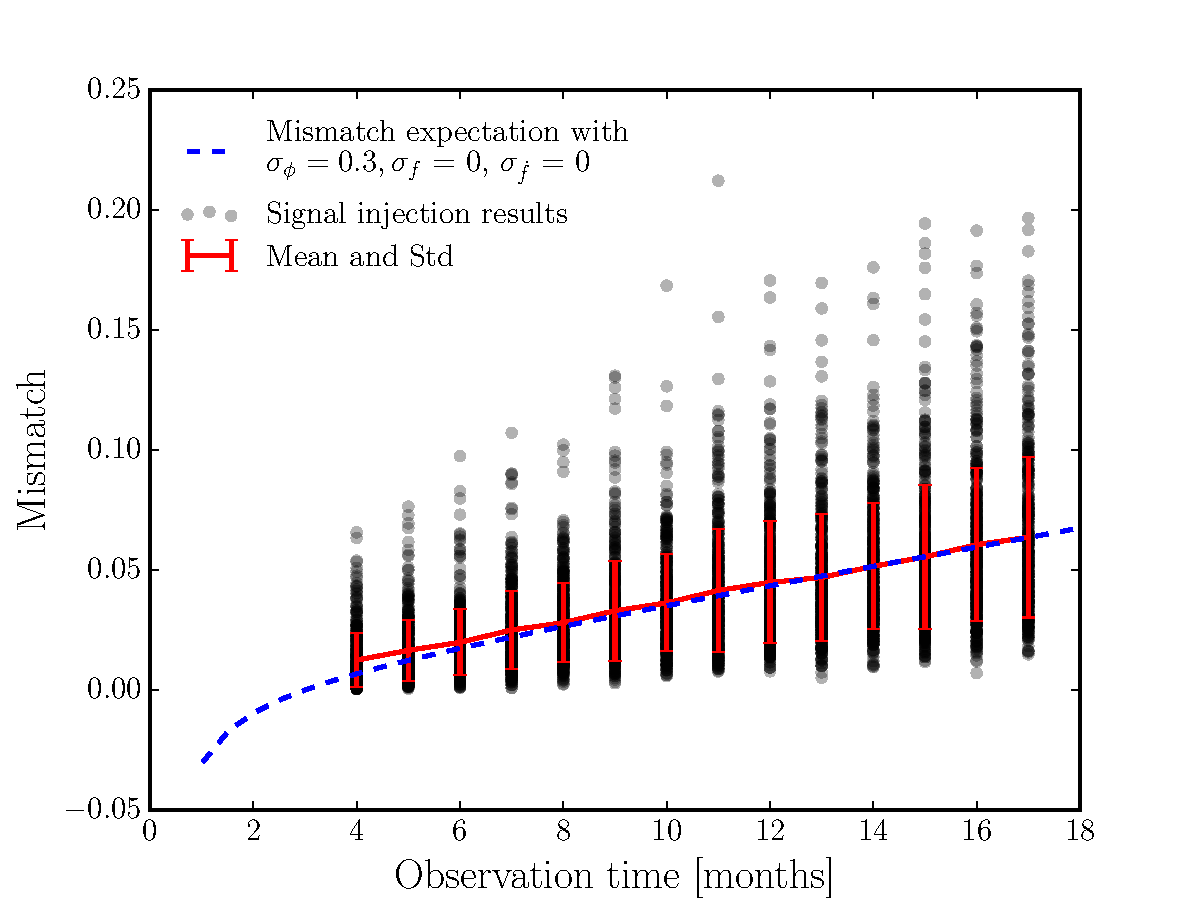
\includegraphics[width=0.5\textwidth]{ExpectationPhase_NarrowBand}}
\subfloat[Random walk in frequency]{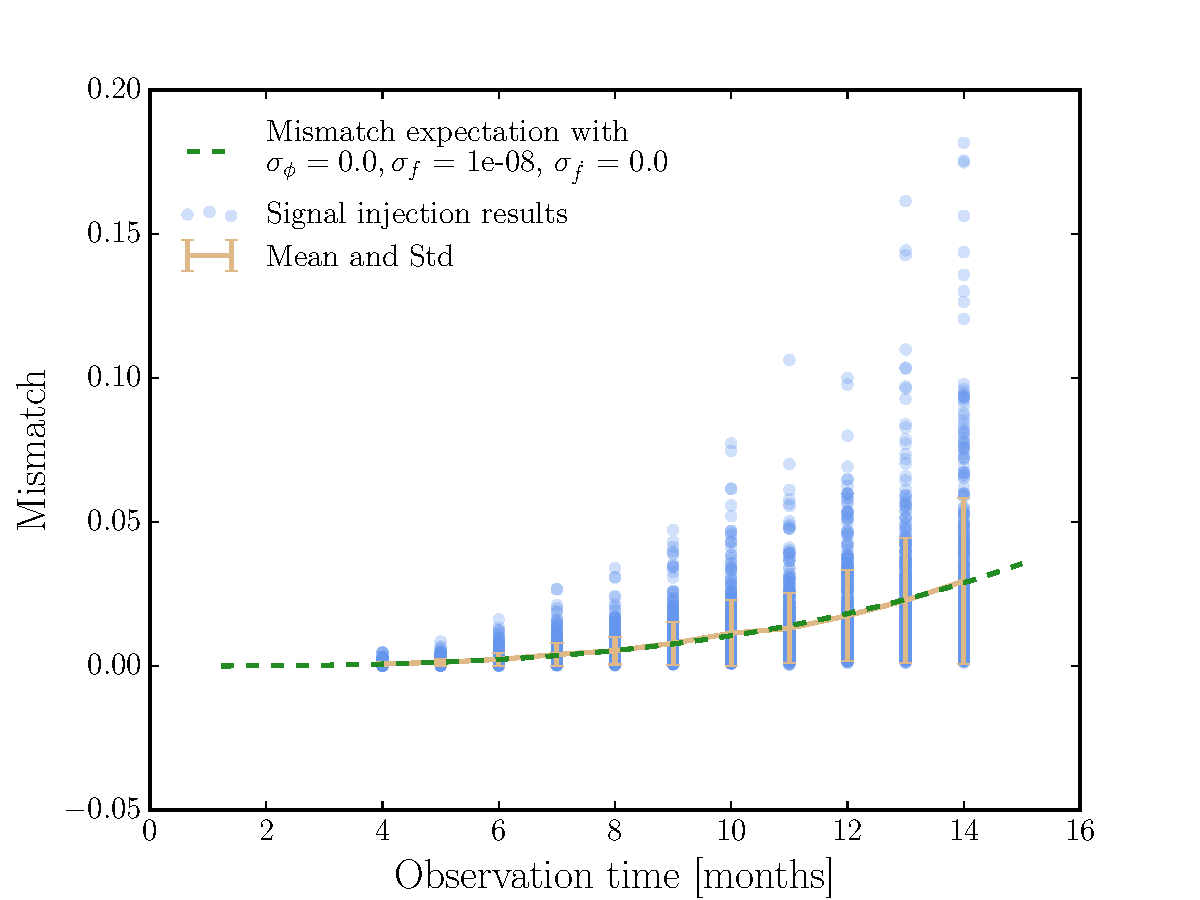
\includegraphics[width=0.5\textwidth]{ExpectationFrequency_NarrowBand}}\\
%\subfloat[Random walk in spin-down]{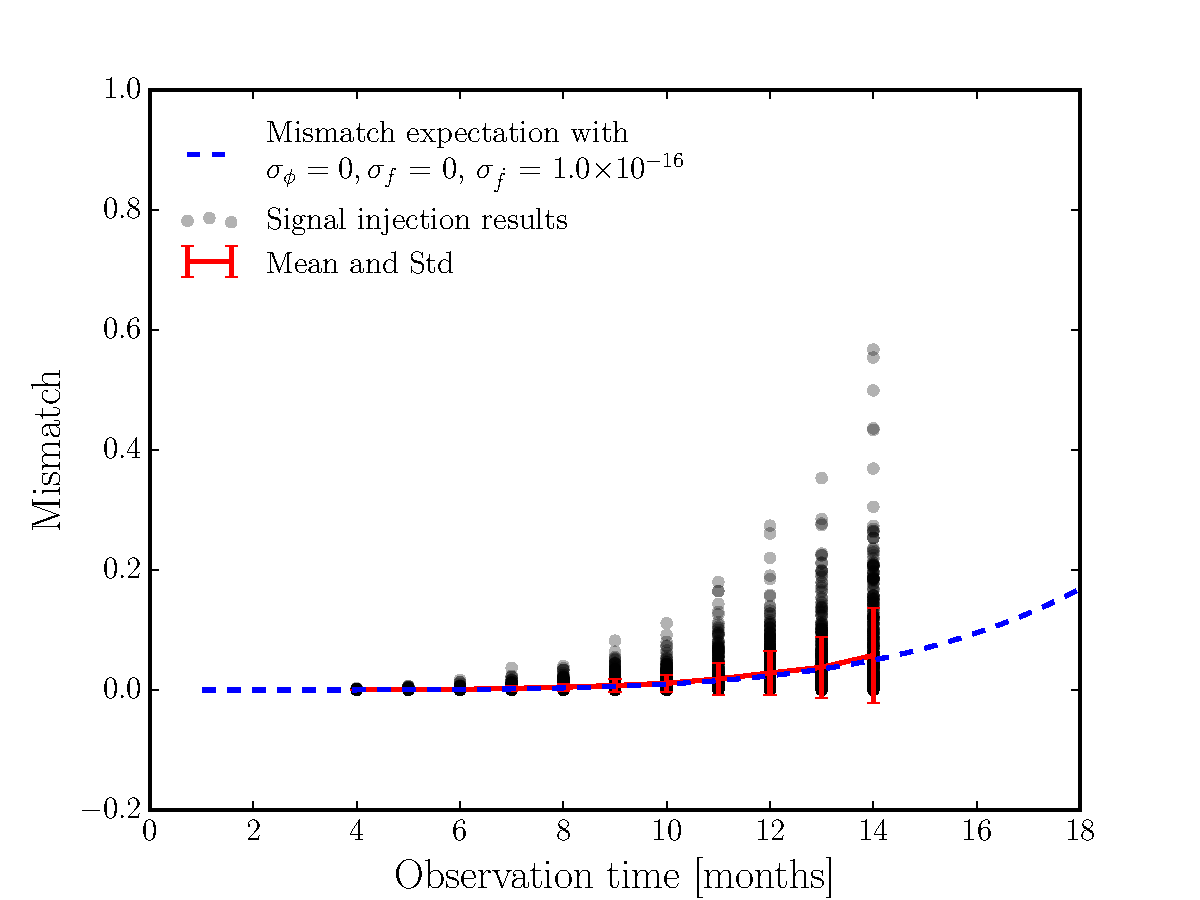
\includegraphics[width=0.5\textwidth]{ExpectationSpindown}}
\caption{A comparison of the Monte Carlo numerical simulated mismatch with the
predictions of Eqn.~\eqref{eqn: Expected mismatch RW in
frequency k2} and Eqn.~\eqref{eqn: Expected mismatch RW in phase k2}; this differs
from Figure~\ref{fig: rw I} in that the numerical mismatch is minimised by selecting
the smallest mismatch from a grid of points in $f_\textrm{t}$ and $\dot{f}_\textrm{t}$.}
\label{fig: verification of minimised RW}
\end{figure}•
\FloatBarrier


\section{Conclusion}

In this section, we have calculated the expectation of the fully-coherent
mismatch when searching for a GW signal which undergoes a random walk in one of
the phase, frequency, or spin-down rate. We did this initially for an
unminimised system and then minimised with respect to the template parameters
$f_\textrm{t}$ and $\dot{f}_\textrm{t}$. In the future, we would like to develop
this work to make direct predictions for GW searches. For example,
searches for GWs from LMXBs assume a constant frequency, but torque fluctuations
could produce a random walk in the frequency; we could model this and, given
an estimate for the random walk parameters, estimate for what observation span
GW searches may be at risk of loosing the signal.

Another observation which we would like to understand further is the
implication of the power-law dependence on the observation time. In particular,
in Eqn.~\eqref{eqn: Expected mismatch RW in frequency k2} we found that for
a random walk in the frequency
$E[\mutilde] \propto \Tobs ^{3}$ while in Chapter.~\ref{sec: timing noise in
cgw} we found that the expected fully-coherent mismatch for timing noise as
described by the Crab ephemeris scales as $\propto \Tobs^{2.88\pm-0.03}$ (see
Eqn.~\eqref{eqn: fit values}). This suggests that the data in Crab ephemeris
may be consistent with a random walk in the frequency (something that was
first noted by \citet{Boynton1972}), but requires further investigation to
establish this.


\begin{subappendices}
\section{Summation identities}\label{sec: summation identities}
\begin{align}
\s{b=1}{c}\s{c=1}{b} X_{c} & = \left( X_{1}\right) 
 + \left( X_{1} + X_{2} \right) + \ldots  +\left( X_{1} + X_{2} 
 + \ldots + X_{c-1} + X_{c}\right)\\
& = c X_{1} + (c-1)X_{2} + \ldots + 2 X_{c-1} + X_{c} \\
& = \s{b=1}{c}(c+1-b)X_{b}
\end{align}•

\begin{align}
\s{j=1}{i-1}\s{k=1}{j-1}(j-k)X_{k} = & [0] + \left[ X_{1}\right] 
+ \left[2X_{1} + X_{2} \right] + \left[3X_{1} + 2X_{2} +X_{3}\right] 
+ \ldots  \\
& + \left[\left(i-2\right)X_{1} + \left(i-3\right)X_{2} 
+ \left(i-4\right)X_{3} + \ldots + 3X_{i-4} + 2X_{i-3} + X_{i-1}\right]  \\
= & \left(1 + 2 + 3 + \ldots +  (i-4) + (i-3) + (i-2)\right)X_{1}   \\ 
& + \left(1 + 2 + 3 + \ldots +(i-4) + (i-3) \right)X_{2}   \\ 
& + \left(1 + 2 + 3 + \ldots + (i-4) \right)X_{3} + \ldots   \\ 
& + (1 + 2 + 3)X_{i-4} + (1+2)X_{i-3} + X_{i-2}  \\
= & \s{k=1}{i-2}k X_{1} + \s{k=1}{i-3}k X_{2}  + \ldots + \s{k=1}{2}k X_{i-3} 
+ \s{k=1}{1}kX_{i-2}  \\
= & \s{j=1}{i-2}\left(\s{k=1}{i-1-j}k\right)X_{j} = 
\frac{1}{2}\s{j=1}{i-2}(i-j)(i-j-1)X_{j}
\end{align}


\section{Least-squares minimisation of a random walk}
\label{sec: least squares minimisation of a random walk}
In this appendix, we will describe the process of fitting and remove a
polynomial from $N$ data points $(y_i, x_i)$ which undergoes a random walk. The
polynomial will be fitted using a least squares minimisation. The $x_i$ are
the independent points at which $y_i$ (which undergoes a random walk) is
measured. We begin by defining the least-squares fitting method then
go on to calculate the residual for several different degrees of polynomial.
This introduces the method in a generic setting which is then applied
in Section~\ref{sec: Random walk models part II} to calculate the mismatch for
a GW signal which undergoes a random walk, but in which the search minimises
the mismatch over the search frequency and frequency derivative.

\subsection{Least square fitting of a polynomial}
%For a full description see
%\url{http://mathworld.wolfram.com/LeastSquaresFittingPolynomial.html}.

Given some data $x_{i}$, $y_{i}$, we define the residual from a least-squares
polynomial fit of order $k$, as
\begin{equation}
    \Delta^{(k)}y_{i} = y_{i} - y^{\textrm{(k)}}_{i},
\end{equation}
where
\begin{equation}
y^{\textrm{(k)}}_{i} = a_{0} + a_{1}x_{i} + a_{2}x_{i}^{2} + \dots
                                                           + a_{k} x_{i}^{k}.
\end{equation}•
Then the residual which we want to minimise is
\begin{equation}
R^{2} = \s{i=1}{N}\left(y_{i} - \left(a_{0} + a_{1}x_{i} + a_{2}x_{i}^{2} +
        \dots + a_{k} x_{i}^{k}\right)\right).
\end{equation}
Partial differentiation with respect to the parameters $a_{i}$, yields $k$
simultaneous equations. Writing these as a matrix and then solving
for the best fit it can be shown \citep{WolframLeastSquares} that
\begin{align}
y^{\textrm{(k)}}_{i} & = X \left(X^{T}X\right)^{-1} X^{T} y_{i} & \textrm{where} & &
X & = \left[\begin{array}{ccccc}
1 & x_{1} & x_{1}^{2} & \dots & x_{1}^{k} \\
1 & x_{2} & x_{2}^{2} & \dots & x_{2}^{k} \\
\vdots & \vdots & \vdots & \vdots & \vdots \\
1 & x_{n} & x_{n}^{2} & \dots & x_{n}^{k} \\
\end{array}\right]
\end{align}
Here $X$ is an example of a \emph{Vandermonde} matrix in which the terms follow
a geometric progression. It is useful to note that
\begin{equation}
XX^{T} = \left[\begin{array}{cccc}
N & \s{i=1}{N}x_{i} & \cdots &  \s{i=1}{N}x_{i}^{k} \\
\s{i=1}{N}x_{i} & \s{i=1}{N}x_{i}^{2} & \cdots &  \s{i=1}{N}x_{i}^{k+1} \\
\vdots & \vdots & \ddots & \vdots \\
\s{i=1}{N}x_{i}^{k} & \s{i=1}{N}x_{i}^{k+1} & \cdots &  \s{i=1}{N}x_{i}^{2k}
\end{array}\right].
\end{equation}

Provided that the $x_{i}$ are suitably defined, then an analytic fit can be
found for any $k$, the difficulty lies in inverting the matrix.

\subsection{Least squares fitting a polynomial to a random walk}
We now take a Gaussian random walk beginning at the origin. To define this let
$\delta y_{i} \sim N(0, \sigma^{2})$ be i.i.r.d.v for which their sum generates
the random walk:
\begin{equation}
y_{i} = \sum_{j=1}^{i}\delta y_{i}.
\label{eqn: ToyModel RW definition}
\end{equation}
We also set each random walk event to occur according to $x_{i} = i \Delta
x$. Then we may define the
residual as the difference between the random walk and a least-squares fit of a
$k^{th}$ order polynomial to the random walk.
\begin{equation}
\Delta y_{i} = y_{i} - y_{i}^{(k)} = y_{i} - X \left(X^{T}X\right)^{-1} X^{T} y_{i}
\label{eqn: fitted residual}
\end{equation}
This suggests the residual will be similar to the random walk, but modified by
the least squares fitting.  To illustrate this, in Figure~\ref{fig: ToyModelRW}
we plot a simulated random walk along with several fits. In the right hand plot
is the corresponding residual; this residual is a random walk that on averaged
will centre around the origin.
\begin{figure}[htb]
\centering
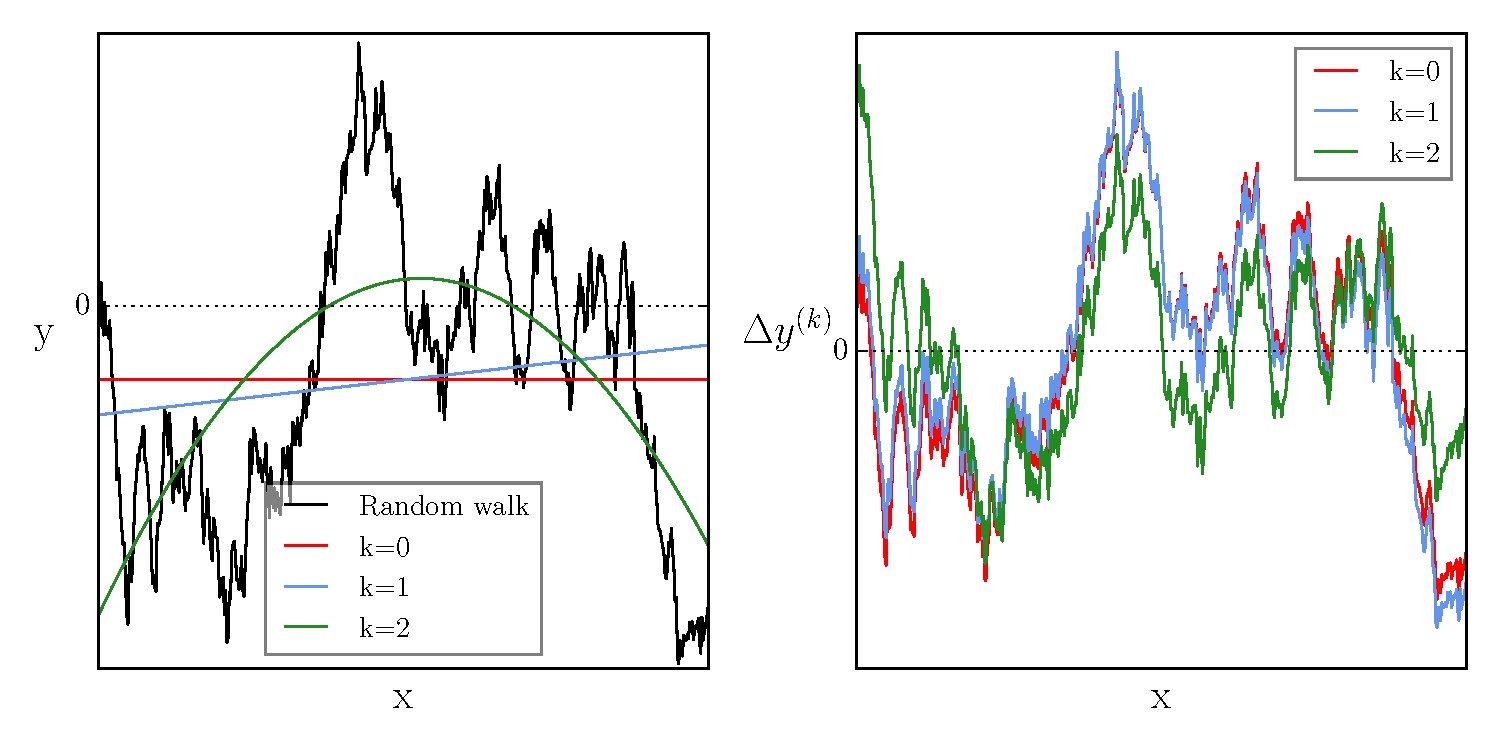
\includegraphics[width=.9\textwidth]{ToyModelRW}
\caption{Example of a random walk on the left along with three polynomial fits
of varying order. On the right is the corresponding residual after subtracting
these fits. A dotted line marks the origin in both plots.}
\label{fig: ToyModelRW}
\end{figure}

\subsection{Zeroth order fitting}

We begin with the case of $k=0$ in which $X^{T} = [1, 1, \dots 1]$ such
that
\begin{equation}
X \left(X^{T}X\right)^{-1} X^{T} = \frac{1}{N} J_{N}
\end{equation}
where $J_{N}$ is the $N\times N$ matrix of ones.  Inserting this into
Eqn.~\eqref{eqn: fitted residual}, the residual from a zeroth order fit is given
by
\begin{equation}
\Delta^{(0)}  y_{i}= y_{i} - \frac{1}{N} \s{j=1}{N}y_{j}.
\end{equation}
The zeroth order residual can be understood as the result of removing the
averaged value.

%For example the
%expectation after $i$ steps of the original random walk can be shown to be
%zero, therefore the expectation for the zeroth order residual after $i$ steps
%will also be zero.

%This can intuitively be understood from the fact that we started out RW at the origin,
%a zeroth order fit shifts the origin but a random walk should

We can now take expectations to understand the behaviour of the residual when
compared to the original definition of the random
walk in Eqn.~\ref{eqn: ToyModel RW definition}. For example, consider
the mean square translation distance from the origin of a random walk after $i$
steps. For a normal random walk, this has the well known result
\begin{equation}
E[y_{i}^{2}] = i \sigma^{2}.
\end{equation}
We can calculate the corresponding quantity of the $k=0$ residual by first
noting that
\begin{align}
E\left[y_{i}y_{j}\right] & = E\left[\s{k=1}{i}\delta y_{k} \s{l=1}{j}\delta y_{l} \right] \\
& = \s{k=1}{i}\s{l=1}{j}E\left[\delta y_{k} \delta y_{l}\right] \\
& = \s{k=1}{i}\s{l=1}{j} \delta_{kl} \sigma^{2} \\
& = \sigma^{2}\min(i, j),
\end{align}
where $\delta_{kl}$ is the Kronecker delta. Then we have
\begin{align}
\left(\Delta^{(0)} y_{i}\right)^{2} & = y_{i}^{2} - \frac{2}{N}\s{k=1}{N}y_{i}y_{k} + N^{-2}\s{k=1}{N}\s{l=1}{N}y_{k}y_{l} \\
& =  y_{i}^{2} - 2 N^{-1} \left(\s{k=1}{i}y_{i}y_{k} + \s{k=i+1}{N}y_{i}y_{k} \right)+ N^{-2}\s{k=1}{N}\left(\s{l=1}{k}y_{k}y_{l} + \s{l=k+1}{N}y_{k}y_{l} \right).
\end{align}
Taking the expectation we have
\begin{align}
E\left[\Delta^{(0)} y_{i}^{2} \right] & = \sigma^{2}\left(i - \frac{2}{N}\left(\s{k=1}{i}k + \s{k=i+1}{N}i \right)+ \frac{1}{N^{2}}\s{k=1}{N}\left(\s{l=1}{k}l+ \s{l=k+1}{N}k \right) \right) \\
& = \sigma^{2}\left(\frac{N}{3} - i + \frac{1}{2} + \frac{i^{2}}{N} - \frac{i}{N} + \frac{1}{6 N}\right).
\end{align}
The expectation after $i$ steps for the residual depends on the length of data
$N$ that was fitted. It can be shown the expectation has a minimum at $i=N/2$.

To gain a better understanding of the difference between the random walk and
the residual random walk, lets consider the sum of squares after $N$ steps for
the random walk
\begin{equation}
E\left[\s{i=1}{N} y_{i}^{2}\right] = \s{i=1}{N} i \sigma^{2} =
                               \frac{1}{2}\left(N^{2} + N\right)\sigma^{2}.
\label{eqn: sum of squares}
\end{equation}
Now we calculate the sum of squares for the residual random walk
\begin{equation}
E\left[\s{i=1}{N} \Delta^{(0)} y_{i}^{2}\right] = \frac{1}{6}\left(N^{2} -1\right)\sigma^{2}.
\label{eqn: sum of squares k0}
\end{equation}
Comparing equations \eqref{eqn: sum of squares} and \eqref{eqn: sum of squares
k0} we note that, for the leading order term, the coefficient is reduced, but
the power remains the same.

%We verify this behaviour with a simple script that produces a random walk of
%length $N$ then fits and subtracts a $0^{th}$ order polynimial; we then
%calculate the sum of the square residual. In Figure~\ref{fig:
%sum_of_squares_res_oth_order} we repeat this operation multiple times then plot
%the average of the sum of squares for the residual while varying $N$, the
%prediction of Eqn.~\eqref{eqn: sum of squares k0} is also plotted showing
%agreement.
%
%\begin{figure}[ht]
%\centering
%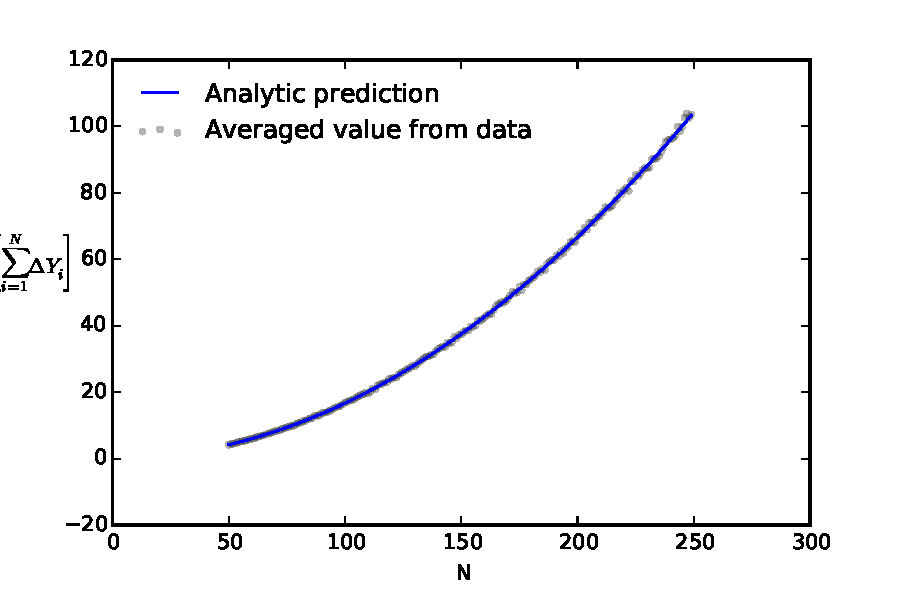
\includegraphics[width=.6\textwidth]{sum_of_squares_res_oth_order}
%\caption{Comparing Eqn.~\eqref{eqn: sum of squares k0} with the averaged sum of squares for a simulated random walk }
%\label{fig: sum_of_squares_res_oth_order}
%\end{figure}

\subsection{First order fitting}
We now consider a first order fitting for which
\begin{align}
y^{\textrm{fit}}_{i} & = X\left(X^{T}X\right)^{-1} X^{T} y_{i} & \textrm{with} &&
X & = \left[\begin{array}{cc}
1 & \Delta x \\
1 & 2 \Delta x  \\
\vdots & \vdots  \\
1 & N \Delta x  \\
\end{array}\right].
\end{align}
Inserting the definitions of $x_{i}$ we can write
\begin{equation}
\left(X^{T}X\right)^{-1} = \frac{1}{N(N-1)}\left[
\begin{array}{cc}
4N+2 & -\frac{6}{\Delta x} \\
 -\frac{6}{\Delta x} & \frac{12}{\Delta x^{2} (N+1)}
\end{array}•
\right] = C.
\end{equation}
For convenience we have defined a symmetric matrix $C$. We then proceed to
define another matrix
\begin{align}
    \mathcal{C}_{ij} & := XCX^{T} \\  & =
\left[\begin{array}{cc}
1 & \Delta x \\
1 & 2\Delta x  \\
\vdots & \vdots  \\
1 & N \Delta x \\
\end{array}\right]
\left[\begin{array}{cc} C_{11} & C_{12} \\ C_{21} & C_{22} \end{array}\right]
\left[\begin{array}{cccc}
1 & 1 & \dots & 1 \\
\Delta x & 2\Delta x & \dots  & N \Delta x
\end{array}\right] \\
& =
C_{11} J_{N} +
C_{12} \Delta x \left[ \begin{array}{cccc}
2 & 3 & \dots & N+1 \\ 3 & 4 & \dots & \vdots \\ \vdots & & & \\  N+1& \dots & \dots & 2N
\end{array}\right] +
C_{22} \Delta x^{2} \left[ \begin{array}{cccc}
1 & 2 & \dots & N \\ 2 & 4 & \dots & \vdots \\ \vdots & & & \\  N& \dots & \dots & N^{2}
\end{array}\right]
\end{align}
We can write $\Delta^{(1)} y_{i}$ as a summation by inferring the dependence of the
$i^{th}$ row of each matrix on the $j^{th}$ column
\begin{align}
\Delta^{(1)} y_{i} & = y_{i} - \s{i=1}{N}\mathcal{C}_{ij} y_{j}
& \textrm{ where} &&
\mathcal{C}_{ij} & = C_{11} + C_{12}\Delta x (i+j) + C_{22}\Delta x^{2} ij
\end{align}

We have now defined the first order residual, we can again compute the expectation
of the $i^{th}$ term
\begin{align}
\begin{split}
E\left[\Delta^{(1)} y^{2}_{i}\right]  =
\frac{1}{15 N \left(N^{2} - 1\right)} &
\left(2 N^{4} - 18 N^{3} i + 9 N^{3} + 78 N^{2} i^{2} - 78 N^{2} i \right.\\
      &\hspace{3mm} + 14 N^{2} - 120 N i^{3} + 180 N i^{2} - 78 N i \\
      &\hspace{3mm} \left. + 9 N + 60 i^{4} - 120 i^{3} + 78 i^{2} - 18 i + 2\right)
\end{split}
\end{align}

Then the expected sum of squares is
\begin{equation}
E\left[\s{i=1}{N} \Delta^{(1)} y_{i}^{2}\right] = \frac{1}{15}\left(N^{2} -4\right)\sigma^{2}
\label{eqn: sum of squares k1}
\end{equation}

\subsection{Second order fitting}
For the residual left after removing a quadratic, the  argument proceeds in much
the same way with
\begin{equation}
C = \frac{1}{N(N-1)(N-2)}
\left[\begin{matrix}9 N^{2} + 9 N + 6 & - \frac{1}{\Delta{x}} \left(36 N + 18\right) & \frac{30}{\Delta{x}^{2}}\\- \frac{1}{\Delta{x}} \left(36 N + 18\right) & \frac{12 \left(2 N + 1\right) \left(8 N + 11\right)}{\Delta{x}^{2} \left(N + 1\right) \left(N + 2\right)} & - \frac{180}{\Delta{x}^{3} \left(N + 2\right)}\\\frac{30}{\Delta{x}^{2}} & - \frac{180}{\Delta{x}^{3} \left(N + 2\right)} & \frac{180}{\Delta{x}^{4} \left(N + 1\right) \left(N + 2\right)}\end{matrix}\right]
\label{eqn: C_2}
\end{equation}•
and
\begin{equation}
\mathcal{C}_{ij} = C_{11} + C_{22}\Delta x^{2}ij + C_{33}\Delta x^{4}i^{2}j^{2} + C_{12}\Delta x(i+j) + C_{13}\Delta x (i^{2} + j^2) + C_{23}\Delta x^{3}(ij^{2} + i^{2}j)
\label{eqn: MCC_2}
\end{equation}
The expression for the expected square value is too long to write out in full
but the expected sum of squares is
\begin{equation}
E\left[\s{i=1}{N} \Delta^{(2)} y_{i}^{2}\right] = \frac{1}{70}\left(3N^{2} -27\right)\sigma^{2}
\label{eqn: sum of squares k2}
\end{equation}•

\subsection{Conclusions}
We now have a method to calculate statistical quantities from the residual
left over after subtracting a $k^{th}$ order polynomial from a random walk.
Considering the sum of squares for a random walk and the residuals in equations
\eqref{eqn: sum of squares}, \eqref{eqn: sum of squares k0},
\eqref{eqn: sum of squares k1}, and \eqref{eqn: sum of squares k2} we find that
the leading order term retains the same
power of $N$ with increasing $k$ but the coefficient of this power gets
smaller. This reflects the improved fitting with the polynomial degrees. We
also note that with each increase in the order of fit we get a limit
on $N$ for which the sum of squares is positive. For zeroth order fitting this
is $N>1$, for first order $N>2$ and for second order $N>3$. This is a result
of using a least squares fitting we need at least $k+1$ points to fit.



\end{subappendices}


\biblio

\end{document}
